\documentclass{sigchi}

% Use this command to override the default ACM copyright statement (e.g. for preprints). 
% Consult the conference website for the camera-ready copyright statement.


%% EXAMPLE BEGIN -- HOW TO OVERRIDE THE DEFAULT COPYRIGHT STRIP -- (July 22, 2013 - Paul Baumann)
% \toappear{Permission to make digital or hard copies of all or part of this work for personal or classroom use is 	granted without fee provided that copies are not made or distributed for profit or commercial advantage and that copies bear this notice and the full citation on the first page. Copyrights for components of this work owned by others than ACM must be honored. Abstracting with credit is permitted. To copy otherwise, or republish, to post on servers or to redistribute to lists, requires prior specific permission and/or a fee. Request permissions from permissions@acm.org. \\
% {\emph{CHI'14}}, April 26--May 1, 2014, Toronto, Canada. \\
% Copyright \copyright~2014 ACM ISBN/14/04...\$15.00. \\
% DOI string from ACM form confirmation}
%% EXAMPLE END -- HOW TO OVERRIDE THE DEFAULT COPYRIGHT STRIP -- (July 22, 2013 - Paul Baumann)


% Arabic page numbers for submission. 
% Remove this line to eliminate page numbers for the camera ready copy
\pagenumbering{arabic}


% Load basic packages
\usepackage{balance}  % to better equalize the last page
\usepackage{graphics} % for EPS, load graphicx instead
\usepackage{times}    % comment if you want LaTeX's default font
\usepackage{url}      % llt: nicely formatted URLs
% llt: Define a global style for URLs, rather that the default one
\makeatletter
\def\url@leostyle{%
  \@ifundefined{selectfont}{\def\UrlFont{\sf}}{\def\UrlFont{\small\bf\ttfamily}}}
\makeatother
\urlstyle{leo}

\usepackage{gensymb}
\usepackage{afterpage}
% see http://tex.stackexchange.com/questions/46055/typesetting-with-inch-symbols-and-sizes-in-inches
% \usepackage{mathpazo}
\usepackage{amsmath}
\def\inch#1{#1''}
\def\ft#1{#1'\thinspace}



% comment macros are in inputmacros.tex
% set up tight list spacing
\usepackage{enumitem} 
\setlist{nolistsep,nosep}

% for toggles
\usepackage{etoolbox}

\newcommand {\studyquote}[1]{\em ``#1''\normalfont}

% CHANGE FROM TOGGLE TRUE TO TOGGLE FALSE FOR NON-ANONYMOUS RENDERING
% http://tex.stackexchange.com/questions/5894/latex-conditional-expression
\newtoggle{anonymous}
\toggletrue{anonymous}
%\togglefalse{anonymous}

% CHANGE FROM TOGGLE TRUE TO TOGGLE FALSE TO HIDE COMMENTS
\newtoggle{comments}
\togglefalse{comments}
%\togglefalse{comments}

% Comment region command (from Wesley Willett)
\usepackage[usenames]{color}
\usepackage[usenames,dvipsnames]{xcolor}
\iftoggle{comments} {
  %if we want to show comments
  \newcommand {\claire}[1]{{\color{Orange}\bf{CT: #1}\normalfont}}
  \newcommand {\sean}[1]{{\color{magenta}\bf{SC: #1}\normalfont}}
  \newcommand {\yang}[1]{{\color{NavyBlue}\bf{YL: #1}\normalfont}}
  \newcommand {\ben}[1]{{\color{violet}\bf{BZ: #1}\normalfont}}
  \newcommand {\bjoern}[1]{{\color{BrickRed}\bf{BH: #1}\normalfont}}
  \newcommand {\achal}[1]{{\color{OliveGreen}\bf{AD: #1}\normalfont}} % can't find another color...
}{
  %if we don't want to show comments
  \newcommand {\claire}[1]{}
  \newcommand {\sean}[1]{}
  \newcommand {\yang}[1]{}
  \newcommand {\ben}[1]{}
  \newcommand {\bjoern}[1]{}
  \newcommand {\achal}[1]{}
}
\newcommand {\systemname}{HOBS }
\newcommand {\systemnamenospace}{HOBS}

% To make various LaTeX processors do the right thing with page size.
\def\pprw{8.5in}
\def\pprh{11in}
\special{papersize=\pprw,\pprh}
\setlength{\paperwidth}{\pprw}
\setlength{\paperheight}{\pprh}
\setlength{\pdfpagewidth}{\pprw}
\setlength{\pdfpageheight}{\pprh}

% Make sure hyperref comes last of your loaded packages, 
% to give it a fighting chance of not being over-written, 
% since its job is to redefine many LaTeX commands.
\usepackage[pdftex]{hyperref}
\hypersetup{
pdftitle={SIGCHI Conference Proceedings Format},
pdfauthor={LaTeX},
pdfkeywords={SIGCHI, proceedings, archival format},
bookmarksnumbered,
pdfstartview={FitH},
colorlinks,
citecolor=black,
filecolor=black,
linkcolor=black,
urlcolor=black,
breaklinks=true,
}

% create a shortcut to typeset table headings
\newcommand\tabhead[1]{\small\textbf{#1}}


% End of preamble. Here it comes the document.
\begin{document}


% as we discussed last time, the "Sees" and "Line-of-sight" suggests some computer vision direction 
% need a different title for sure, but not in a hurry
\title{Head orientation-based target selection in physical spaces}
%Project GlasSees: Direct Interaction Through Line-of-sight}

\iftoggle{anonymous}{
\author{
 \alignauthor Anonymous for submission\\
    \affaddr{...}\\
    \email{...}\\
  }
}{ %else
  \numberofauthors{1}
  \author{
  \alignauthor Yu-Hsiang Chen$^{\dagger}$, Ben Zhang$^{\dagger}$, Claire Tuna$^{\dagger}$, Yang Li$^{\ddagger}$, Edward Lee$^{\dagger}$, Bj\"orn Hartmann$^{\dagger}$ \\
  \affaddr{$\dagger$: UC Berkeley EECS \& CITRIS Invention Lab \hspace{0.25in} $\ddagger$: Google Research}\\
  \email{sean.yhc@gmail.com, benzh@eecs.berkeley.edu, clairetuna@gmail.com, yangli@acm.org, eal@eecs.berkeley.edu, bjoern@eecs.berkeley.edu}
  }
}

\maketitle

\begin{abstract}
\bjoern{I prefer to write the abstract {\em first}, not last, as a blueprint for the rest of the paper.}

Emerging head-worn computing devices can enable hands-free interactions in physical spaces. 
%
We introduce and characterize a method for selecting and interacting with physical targets at a distance using head orientation. We augment a commercial wearable device, Google Glass, with an infrared (IR) emitter to select targets equipped with IR receivers. The fundamental imprecision of head orientation requires a large selection beam \bjoern{term?} for successful target acquisition. However, a large beam area can lead to ambiguous selections. We introduce a two level disambiguation strategy: first, networked receivers use IR intensity sensors to estimate which target is the intended selection; second, users can fall back to a manual disambiguation technique using their near-eye display. The technique does not require an a priori map of target devices. However, a spatial data structure can be inferred to overcome sensor saturation problems in environments hostile to IR communication (e.g., in sunlight).
%
A target acquisition study with 14 participants shows that selection using head orientation with our device outperforms list selection on a wearable device. Intensity-based target disambiguation reduces selection time and error rate in dense target environments. We apply this technique to an application for controlling smart appliances and report qualitative usage data from a smart home scenario.

\end{abstract}

\keywords{
  Wearable computing; tangible; smart devices; remote control; glass; infared
}

%% refer to http://www.acm.org/about/class/ccs98-html
\category{H.5.2.}{Information Interfaces and Presentation (e.g. HCI)}{Interaction styles (e.g., commands, menus, forms, direct manipulation)}.

\vfill\eject

\section{Introduction}
\label{sec:introduction}

There has been the vision of smart-home and smart-office where everything around is intelligent enough to assist human in everyday life. The development of radio technology, sensors, and actuators are making this dream come true. You can buy those basic components online \cite{SmartHome, NinjaBlocks} and many hobbyists have already created their own smart environment (see \cite{BRAD} as an example). Recently, with the the prevalence of smartphones, many systems \cite{SmartThings, Lockitron} have been integrated into smartphone applications to lower the barrier for ordinary users.

Admittedly, people have been used to accessing the Internet, conversing with friends, and even dealing with online business through their smartphones. These handheld devices serve as an important portal for users to be connected to the Internet. And now many systems are making smartphones the portal to interact with physicalworld. Given all the benefits we can get by using smartphones -- networking,  display, gesture input, and increasing computability,  we argue that traditional GUI on mobile platform still imposes difficulty in interacting with physical objects. Take iPhone for example, users are required to browse a list of possible icons and then select the right one. Even on Android platform, you can create widget to simplify the browsing overhead. We hold the opinion that squeezing physically distributed objects onto a-few-inch screen is not the right approach. And a more direct approach is desirable.

In this project, we aim to explore the ability of direct interaction by using glass-based attention tracking to pin-point the target. 

% explain why we need glass form factor


The rest of this paper is structured as follows. In Sec.\,\ref{sec:related-work}, we will give an overview of some related projects. Then we present our approach in detail about the system design and implementation in Sec.\,\ref{sec:design} and Sec.\,\ref{sec:implementation} respectively. Then Sec.\,\ref{sec:evaluation} shows our evaluation results and we provide an in-depth discussion (Sec.\,\ref{sec:discussion}) about different kinds of interaction since not all are suitable for our system. Sec.\,\ref{sec:conclusion} concludes this paper.


%%% Local Variables: 
%%% mode: latex
%%% TeX-master: "main"
%%% End: 

%!TEX root = uist14.tex
\section{Background and Related Work}
\subsection{Head and Eye Input}
Head movement has long been used for virtual camera control in VR applications~\cite{pausch_user_1993} and as an assitive input technology for cursor control of desktop applications~\cite{}. Head joysticks have been evaluated using Fitts' law and \bjoern{what did they find?} However, 
Card, summarizing other work, shows that neck muscles are a poor muscle group for pointing in general: neck muscles only have a bandwidth of about $4.2bits/s$ (compared to $23bits/s$ of wrist muscles used by a standard mouse)~\cite{Card:1991:MAD:123078.128726}. 

Contrast: we're not working on GUI tasks, but on identifyign and selecting ubicomp objects in physical spaces.

Gaze control of existing graphical user intefaces~\cite{kumar2007eyepoint}. There are also wearable gaze trackers~\cite{SMI} -- but while these can provide a concrete point in space where a user is looking, turning this information into a selection information requires either a fixed absolute map of each space with known location and orientation of the user, or... Our system works through point-to-point IR communication and does not require any a priori knowledge of where objects are located.

Our work is closer in spirit to Selker's headworn system~\cite{Selker:2001:EGE:634067.634176}.

\subsection{Area Cursors}
A central hypothesis of this paper is that the area selection paradigm is well matched to head orientation input.
\bjoern{Need a discussion of area cursors~\cite{kabbash1995prince,worden1997making,Findlater-uist2010}.}

\subsection{Pointing in physical spaces}
\bjoern{take this from prior CHI submission.}

\bjoern{TODO: Add discussion of ~\cite{swindells_that_2002,merrill_augmenting_2007}.}

%\bjoern{removed background - folded into related work.}
%\section{Background}
%\label{sec:background}


%% Bjoern: I would mostly rely on prior literature here. There are neck-controlled joysticks for users with disabilities that are probably useful to look at. see below.
 
%% YL: I also think we should briefly cover how people used to detect head-orientatation. I don't have references at hand and the only paper I can recall is Michel's paper. I think Pourang Irani has papers in this area too. Overall I think previous ways are too heavyweight. In comparison, your way of acquiring head orientation is more effective and lightweight.

%In this section, we will first provide some background about human's neck muscle kinectics. Given that constrain, we think the right way to achieve head-orientation based targeting should be using the area selection technique. This motivates our selection of using IR to capture users' head orientation and also the carefully design of the disambiguation technique.



%%% Local Variables: 
%%% mode: latex
%%% TeX-master: "uist14"
%%% End: 

%!TEX root = uist14.tex
\section{Iteration 1: IR-based Head Orientation with List Refinement}

\subsection{Interaction Flow}
\bjoern{I pulled this from the earlier paper}

\begin{figure}[t!]
\centering
\includegraphics[width=\columnwidth]{figures/stepbystep_small.png}
\caption{Targeting interaction: when users turn towards a controllable appliance (A$\rightarrow$B), the appliance shows immediate visual feedback (red LED) (B). Users confirm that they wish to connect to this appliance with a tap (C) which triggers connection feedback (blue LED) on the appliance.}
\label{fig:interaction}
\vspace{0.1in}
\includegraphics[width=\columnwidth]{figures/stepbystep_multi_small.png}
\caption{When multiple appliances are within range, they all have red LEDs illuminated for feedback (A). When users initiate connections, all target appliances toggle on blue LEDs while the currently selected one blinks (B). Swiping on the touchpad traverses among responding appliances (C).}
\label{fig:interaction_multi}
\end{figure}

\begin{figure}[t]
\centering
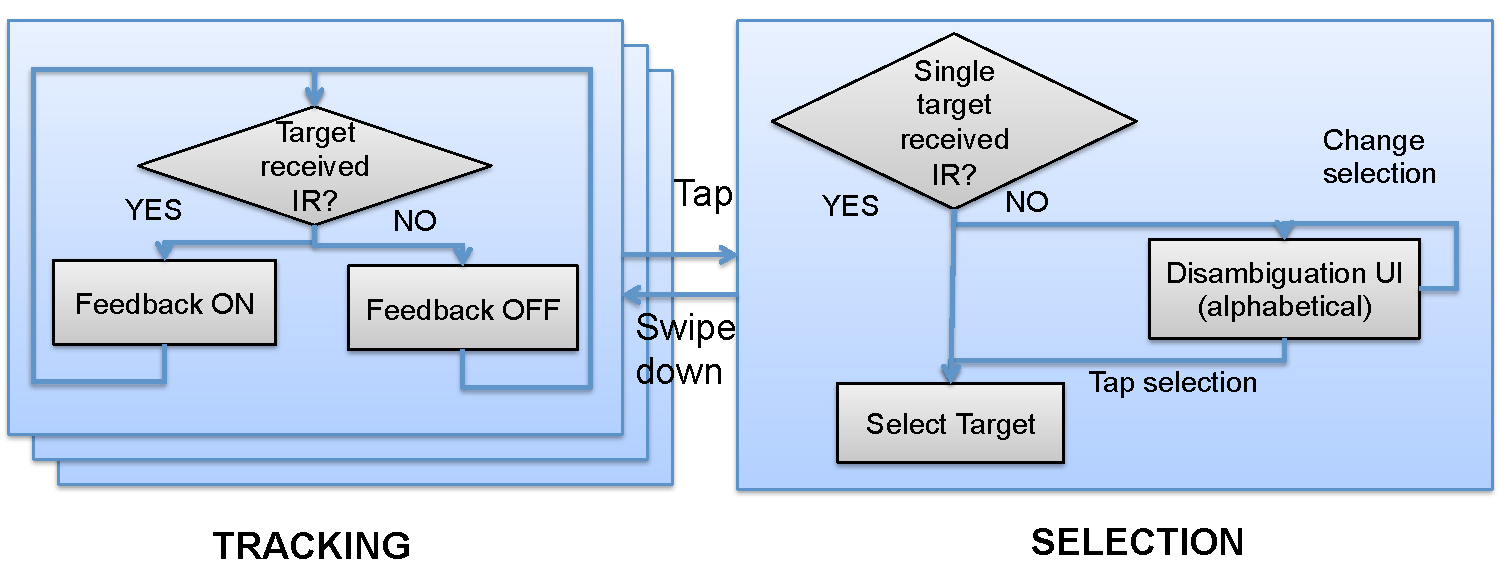
\includegraphics[width=1.0\columnwidth]{figures/selectflow01.pdf}
\caption{Head orientation selection flowchart for our first design.}
\label{fig:selectflow01}
\end{figure}

{\bf Look:} Users looking in the general direction of the intended target.
Glass periodically sends a device id through its IR emitter analogous to Patel's approach~\cite{patel_2-way_2003}. Target appliances have IR receivers and offer immediate visual feedback by toggling a red LED whenever a valid id is received (Figure~\ref{fig:interaction}B). This enables {\em scanning} the environment with one's gaze to see which appliances can be controlled.

{\bf Initiate:} Users confirm their desire to connect to an appliance by tapping on the Glass touchpad. After they are connected, the target appliance toggles on a blue LED as visual feedback (Figure~\ref{fig:interaction}C). The next section on disambiguation deals with cases in which multiple appliances received valid IR signals. At this point, all further communication switches over to the 802.15.4 wireless network so that line of sight to the target is no longer needed.

{\bf Refinement:}
Head orientation only indicates a general area of visual interest. It does not necessarily match gaze orientation as extra-ocular muscles can move the eyes. The IR beam of our device also has a certain spread . In an environment dense with potential targets, multiple targets could be within range. Users can tell when multiple feedback LEDs in the environment illuminate (Figure~\ref{fig:interaction_multi}A). To disambiguate, users can either move to adjust their head position, or, alternatively, call up a disambiguation dialog on the Glass display. The dialog presents a list filtered to only those appliances that are within IR range, while appliances also use blue LED as visual cues: all responding appliances light up LEDs while the currently selected one blinks (Figure~\ref{fig:interaction_multi}B). Users navigate the list using the touchpad (Figure~\ref{fig:interaction_multi}C), and then continue their interaction as described above.

\subsection{Implementation}
\begin{figure}[t]
\centering
\includegraphics[width=0.7\columnwidth]{figures/tube_from_top.jpg}
\caption{Our augmented Glass prototype has a frame-mounted infrared emitter.}
\label{fig:glass}
\end{figure}
\begin{figure}[t]
\centering
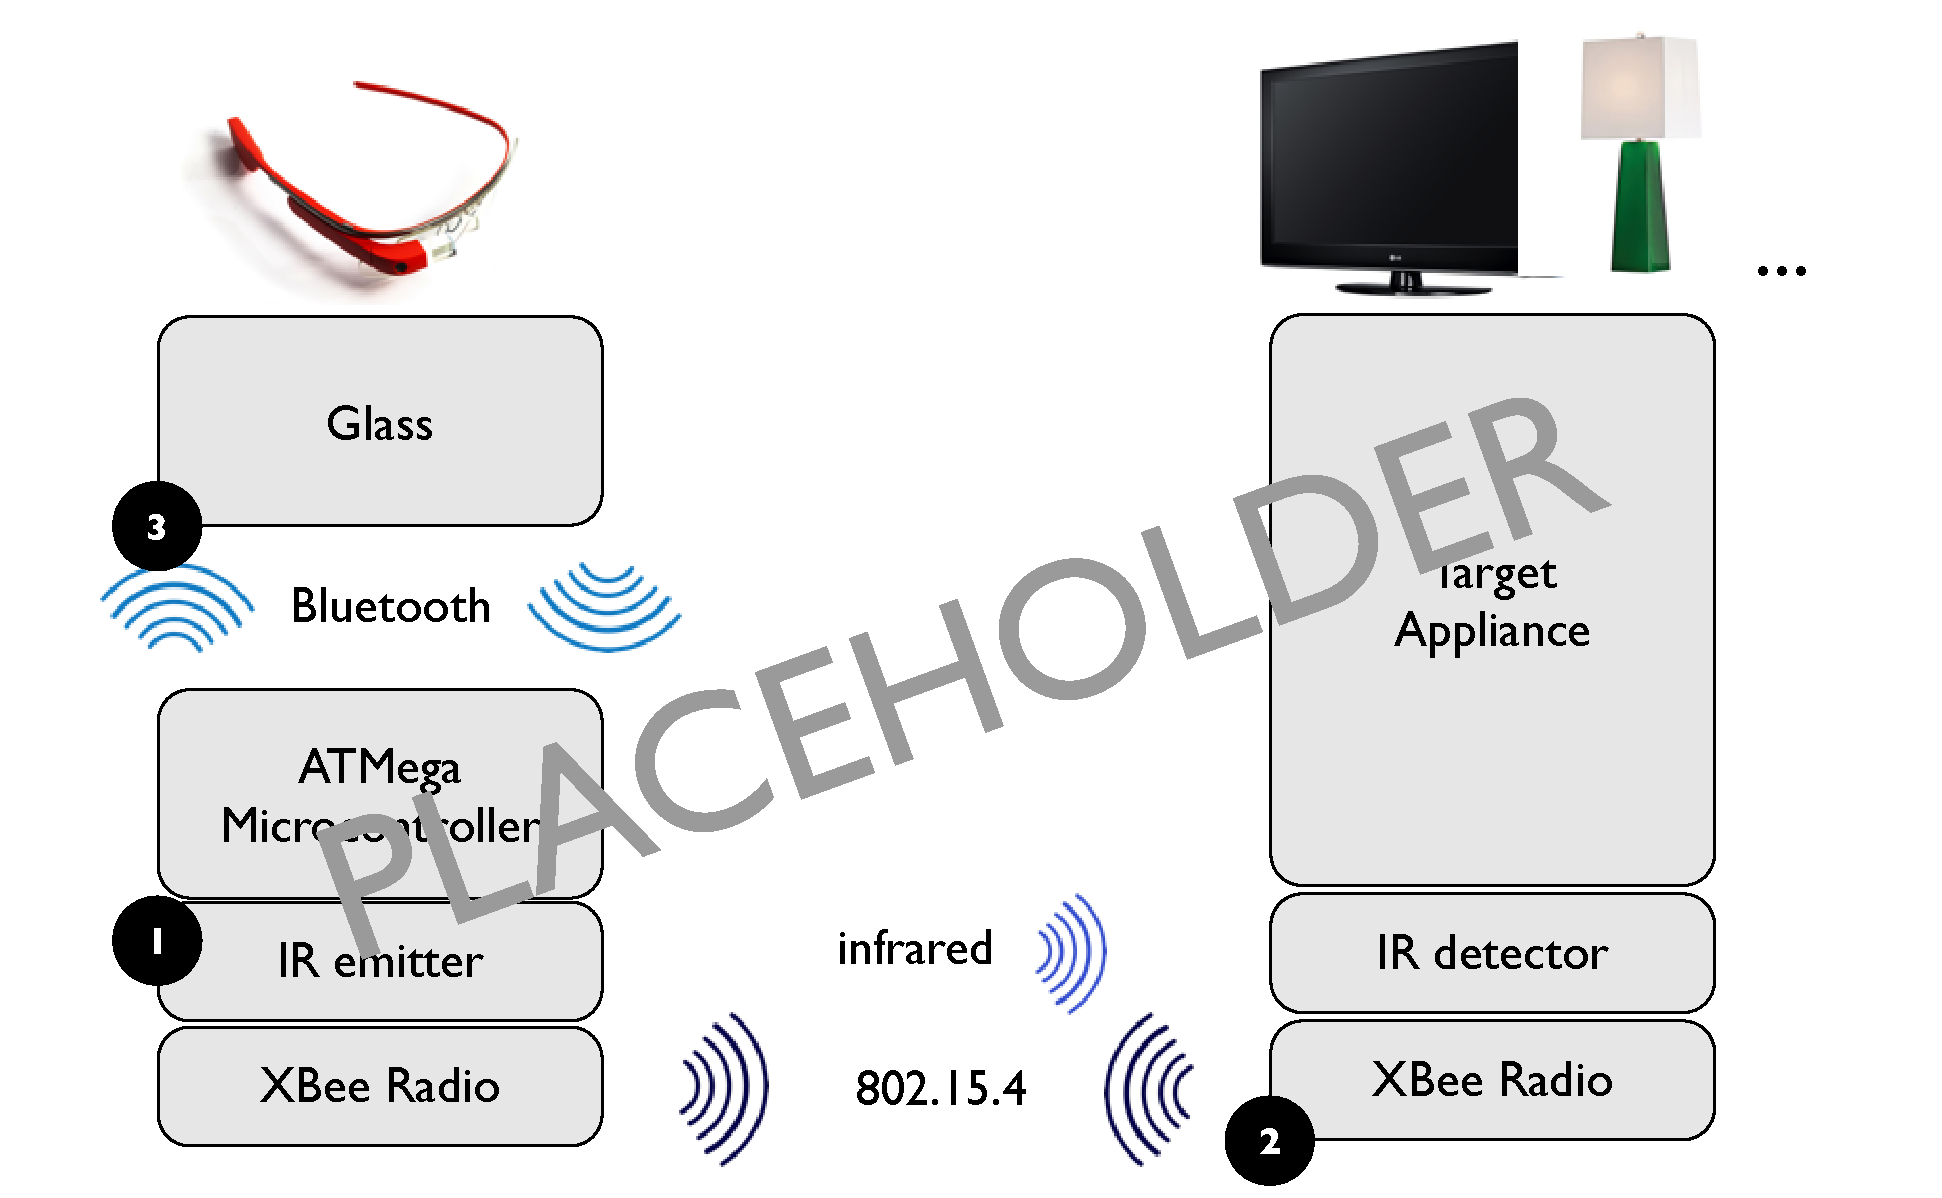
\includegraphics[width=1.0\columnwidth]{figures/architecture}
\caption{In our system architecture, selection is initiated through infrared but confirmed over 802.15.4. This permits wearers to move their head freely after connecting to an appliance. In the research prototype, users have to carry an additional microcontroller board that marshals messages between Glass' Bluetooth radio an IR/802.15.4, but our custom hardware could also be integrated into the wearable device.}
\label{fig:architecture}
\end{figure}

Our prototype consists of a Google Glass Explorer Edition device, augmented with an infrared emitter that is mounted on the frame, pointing out in the direction of the wearer's view (Figure~\ref{fig:glass}). The IR emitter LED is mounted in a \bjoern{3D printed housing which can be adjusted so the emitter can point straight forward for different head shapes}.

Our measurements suggest that IR communication can be targeted to an area about 60-120cm in diameter, up to 5m in front of the user. These values are a reasonable match for selecting targets in a room-size environment. A wider beam would lead to an increased chance of multiple appliances receiving IR signals simultaneously. A narrower beam will make targeting more challenging, given the precision constraints of human head movement.

In our prototype, Glass communicates over Bluetooth to an additional microcontroller board the user has to wear (Atmel ATMega256). This board marshals XBee to Bluetooth messages in both directions and also controls the IR LED mounted on the Glass frame (Figure~\ref{fig:architecture}). This architecture was chosen for reasons of expediency and we do not claim optimality for our design decisions. Future head-mounted devices could clearly integrate IR emitters; the choice of local wireless technology could also change. In particular, one could substitute WiFi modules or design an all-Bluetooth network.


\subsection{Device Characterization}
We determined the usable range and accuracy empirically with one IR emitter and two IR receivers. The IR emitter constantly sent out an id signal. The receivers that correctly received the signal turn their LED on for 300 ms. Our measurements suggest that IR communication can be targeted to an area about 2--4' in diameter, up to 16' in front of the user. These values are a reasonable match for selecting appliances in a room-size environment. A wider beam would lead to an increased chance of multiple appliances receiving IR signals simultaneously. A narrower beam will make targeting more challenging, given the precision constraints of human head movement.

%!TEX root = uist14.tex
\section{Study 1: Physical Target Acquisition Study}
To understand the accuracy and performance of head-orientation-based selection through our device, we carried out a comparative target acquisition study, where participants had to connect to wireless nodes distributed in a room with our technique, and with an alternate list selection approach.


\subsection{Apparatus}
In an indoor environment, 10 wireless nodes are spread across a room (Figure~\ref{fig:targeting-study-layout}). Each node is an embedded wireless system with a microcontroller, IR receiver, a wireless XBee radio, and three status LEDs %(Figure~\ref{fig:target}). %An yellow LED indicates that the device is the target that should be selected in the current trial; a red LED lights up whenever the device receives an IR signal from Glass; a blue LED shows when participants have successfully connected to a device, and is also used for disambiguation when multiple targets are within IR range. 
Next to each target, a paper sheet shows a number and letter combination, which is used for uniquely identifying the device. The numbers are the primary identifiers, ordered from left to right in the room. 

\begin{figure}[t]
\centering
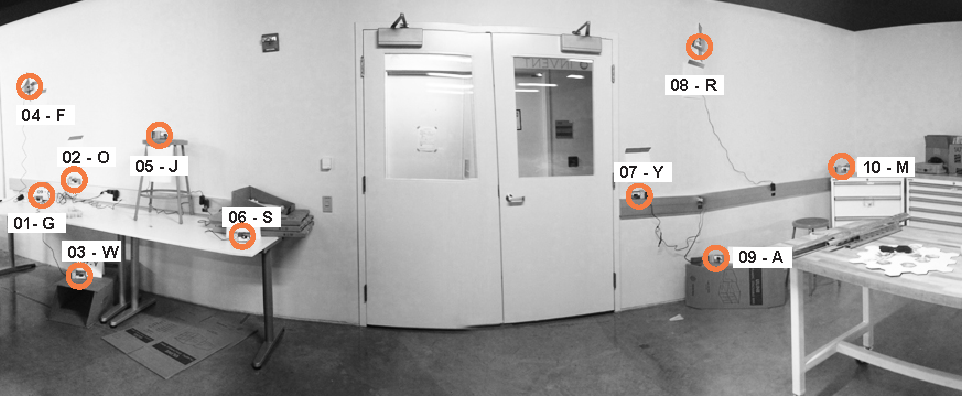
\includegraphics[width=1.0\columnwidth]{figures/targeting-study-layout.pdf}
\caption{In the targeting study, participants had to find and select one of 10 targets in a lab environment. Targets were called out by number; for the list mode condition, participants need to match numbers to letters.}
\label{fig:targeting-study-layout}
\end{figure}
%\begin{figure}[b]
%\centering
%\includegraphics[width=0.8\columnwidth]{figures/study-node.pdf}
%\caption{An example node from the targeting study --- we constructed 10 such nodes - each mounted in a box.}
%\label{fig:target}
%\end{figure}

\subsection{Methodology}
In our within-subjects design, participants performed 15 target acquisition tasks each with two interaction styles. In the {\em infrared} mode condition, participants used our IR targeting approach; in the {\em list} mode condition, participants had to look up a device's letter code on the printed paper next to the device and then select that letter code from a list displayed on their Glass device. The list was navigated with swipe motions on the Glass touchpad. For each task, participants started at a fixed position in the room. The experimenter called out a number and simultaneously started a timer. Participants then had to find the corresponding device (by looking for its printed code). In the {\em infrared} mode, participants then selected and acquired the target by aiming the IR beam at the target, and confirmed their selection with a touch pad tap. If more than one target was within range, participants had to either use the disambiguation dialog or reposition themselves. In the {\em list} mode, participants had to read the letter next to the number and then select that letter by browsing a linear list shown in their Glass display. While the list was alphabetized, letter arrangement in the room was not. This design required participants to find the target in the room before starting a list navigation to keep visual search times similar in each condition.

Afterwards, participants completed a survey that elicited answers to Likert-scale questions as well as open-ended answers about their experience.

\subsection{Participants}
We recruited 14 participants from our institution. 13 had never used Glass before. 4 wore prescription glasses, which may have affected their task performance as wearing glasses beneath Glass makes it more cumbersome to secure the position of Glass and to adjust the screen to the optimal angle. Half of them performed {\em infrared} mode first and the other half did {\em list} mode first.

\subsection{Measures}
The main measures were {\bf target acquisition time}: the time required to identify, select, and connect to a wireless target device; and {\bf user preference}: which interface users preferred for the task after completing the study.

\subsection{Results}
\subsubsection{Performance data}
The time to complete each task can be broken down into the following pieces:

$t_{infrared}=t_{locate}[+t_{reorient}][+t_{disambiguate}]+t_{tap}$

$t_{list}=t_{locate}+t_{listnav}+t_{tap}$

In both conditions, participants first have to locate the target announced by the experimenter through visual search ($t_{locate}$). In the {\em infrared} mode, participants may then directly confirm their selection if only a single target was selected ($t_{tap}$). However, if they don't immediately receive feedback that their target was selected, or if multiple targets were selected, users either have change their position or head orientation ($t_{reorient}$) or they have to step through the on-screen disambiguation dialog ($t_{disambiguate}$). In the {\em list} mode, participants must scroll through the list to find the desired target identifier ($t_{listnav}$).
Thus, {\em infrared} will show a performance benefit if $(t_{reorient}+t_{disambiguate})<t_{listnav}$. This depends on the number of total devices in the environment (increasing $t_{listnav}$), and their density (which will increase $t_{disambiguate}$). 

\begin{figure}[t]
\centering
\includegraphics[width=1.0\columnwidth]{figures/R_time_by_Category.pdf}
\caption{Boxplot of task completion times for the comparison between {\em infrared} mode and {\em list} mode (A), and between IR multiple responses cases and IR single response cases (B). The centers of boxes are median values, while white dashed lines are mean values.}
\label{fig:selection-times}
\end{figure}

We first show results for 10 targets and then discuss extrapolations of these results. Average target acquisition time $t_{infrared}$ was 6.67 seconds, while $t_{list}$ was 8.86 seconds (Figure~\ref{fig:selection-times}A). This difference is significant (Student's t-test, $t(279)=-3.81, p=0.00017$). % \bjoern{you need to report the t statistic and degrees of freedom as well - t(df)= n,p=m.} 

To further understand the performance gain in {\em infrared} mode, especially the factor $t_{disambiguate}$, we compare selection times when multiple devices are targeted (and disambiguation is required) to single-device selection times (Figure~\ref{fig:selection-times}B). When there is a single device, $t_{disambiguate}$ is 0 and it takes 6.40 seconds (on average) to complete the connection. When multiple devices are in range, the time increases to 9.16 seconds, indicating 2.76 seconds required to disambiguate. Though it takes significantly longer ($t(19)=-2.7827, p=0.012$ using t-test) in the {\em multiple} case, these cases made up only 10\% of total infrared trials.
%, even we intentionally placed a few devices nearer to each other. % 19 / (19+168 )

\begin{figure}[t]
\centering
\includegraphics[width=1.0\columnwidth]{figures/R_List_by_Target.pdf}
\caption{Times taken to select a device vs.~its order in the list. The dotted line is a linear fit between the mean times and device orders. Two horizontal lines of mean target acquisition times in {\em infrared} mode are also annotated for comparison.}
 % \bjoern{Add horizontal lines at $t_{IRsingle}$ and $t_{IRmultiple}$.}
\label{fig:time-vs-list-order}
\end{figure}

For each device, $t_{listnav}$ depends on their relative position in the list. Figure~\ref{fig:time-vs-list-order} shows the time it takes to select a device (means and standard deviations) as a function of its list position - the trend line (dotted) enables extrapolation to estimate at what number of devices the {\em infrared} mode interaction techniques will outperform {\em list} mode\footnote{The higher mean value at $order=1$ is caused by one outlier when the participant tried multiple times in {\em list} mode to connect to the right target.}. From the figure, we can see that once the target's order has increased to be larger than 6, the average $t_{listnav}$ for that target would be larger than $t_{reorient} + t_{disambiguate}$. We expect that, when the number of targets keeps increasing, there would be larger time reduction in {\em infrared} mode.

% \bjoern{A linear trend is visible, and the regression returns with coefficient of determination ($R^2=0.032$). --- This R value is basically no correlation at all! try to run a correlation only on the median times. }

Participants' selection errors do occur in both conditions. However, error rates were low (1.1\% in {\em infrared} mode, and 2.9\% in {\em list} mode, respectively). This precludes us from running a more detailed analysis. 


%\subsubsection{Preference}

%Eleven of 14 users preferred infrared mode over list mode (three preferred list, one was undecided). While both interfaces were judged similarly on overall ease of connecting, list navigation was also perceived to be cumbersome. As self-report data can easily skew positive as participants try to please experimenters, we also asked participants to elucidate why they preferred one interface over the other.

%List mode had certain advantages: It was judged to be more accurate and predictable as there was always exactly one device selected in the list (\studyquote{With the list you never have to worry about accidentally picking up two targets}). Also, it did not require a clear line of sight to the target device so participants did not have to move from their starting position (\studyquote{The shortcoming of the IR mode was that you had to be a certain distance away in order for it to detect the appliance}). 

%On the other hand, list mode was judged to be more \studyquote{annoying} and tedious. The temple-based touchpad for selection was difficult to use for a participant with long hair: \studyquote{List mode was physically difficult for me to navigate, since my long hair wasn't tied back and it kept interfering with my swiping.} Another participant also commented on the ergonomic challenge of touchpad use on Glass: \studyquote{The strength of the IR mode was that I didn't have to use my fingers as much to control. If the items were spaced relatively far apart, it was easy to select a specific appliance.}

%One noted benefit of infrared mode was a feeling that it was \studyquote{more direct [than list mode]}, allowing users to focus on the targeted objects instead of the screen. One subject called it \studyquote{natural to interact with things just by looking at them}. Another mentioned that \studyquote{it's really convenient that what I'm looking at is what I'm targeting}. 

%A few perceived weaknesses of infrared mode were the necessity to move the head in order to control a device and the imperfect mapping of gaze to target. One participant said that it was \studyquote{awkward to be aiming your head at things, tweaking back and forth to get it right}. Another noted that observing the head movement didn't capture the site of her attention, because \studyquote {eye movement is an important part of how people look around}. Users had to learn the usable angle of the IR emitter before they became successful at controlling the devices: \studyquote{I had to compensate by tilting my head up a little bit.}
%!TEX root = uist14.tex
\section{Iteration 2: IR Intensity refinement}

\bjoern{The results of the first study show that head orientation targeting can outperform linear list selection, but that disambiguation (or refinement step, need to decide on consistent terminology) is costly.

Our approach to avoid paying this penalty is to provide more information to the system which target is more likely than another to be the intended selection. We do so by collecting received IR signal strength at each target node and comparing measurements of all candidate targets.}

\subsection{Interaction Flow}
\bjoern{
Intensity data is used in two ways (see Figure~\ref{fig:selectflow02}): 1) the difference in intensity between the strongest and second target exceeds a threshold, the target with the strongest received signal is automatically selected; 2) if the difference falls below the threshold, the refinement UI from the previous iteration is displayed, but items are ordered in decreasing intensity. This should maximize the chance of being able to confirm the intended target without additional UI navigation actions}.


\begin{figure}[t]
\centering
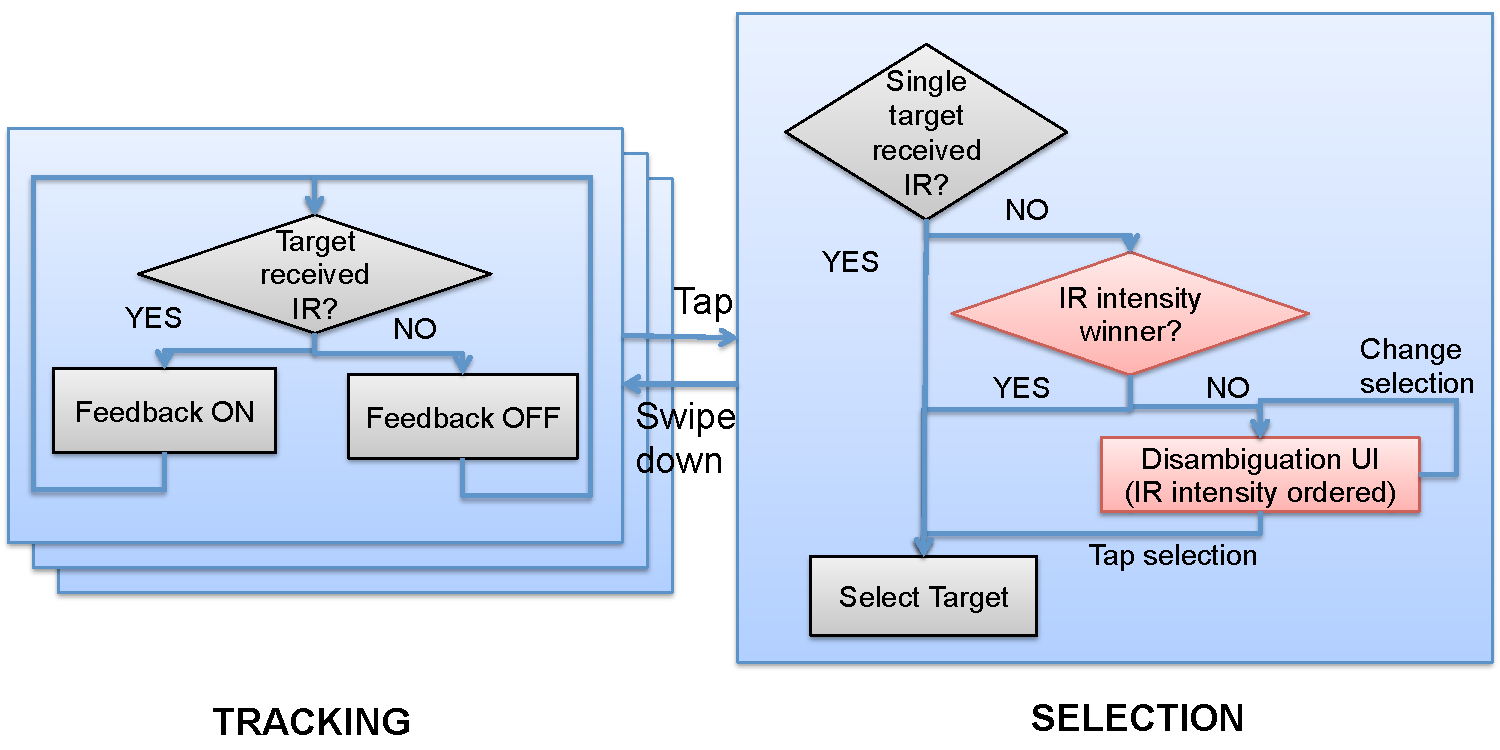
\includegraphics[width=1.0\columnwidth]{figures/selectflow02.pdf}
\caption{Head orientation selection flowchart for our second design with IR intensity measurement.}
\label{fig:selectflow02}
\end{figure}

\subsection{Implementation}
\bjoern{we use sensor X and LED y which give useful readings at up to N feet. Intensity falls of as $1/d^2$ with distance and approximately $xyz$ with angle. We empirically set the threshold for automatic selection without refinement at Z.}\bjoern{maybe show some measurements for intensity based on distance and angle as we had discussed a while ago. not essential. }

%!TEX root = uist14.tex
\section{Study2: Benefits of IR Intensity refinement}
\bjoern{write this with analogous structure as study 1 and focus on the comparisons we discussed:
1) Chi-square test of required refinement dialogs; 2) chi-square of number of times the first item in the UI was appropriate; 3) t-test of selection times; 4) comparison of error rates (likely, IR will be higher - that's the price to pay for a smarter technique).}

%!TEX root = uist14.tex
\section{Iteration 3: Orientation-based refinement}
\bjoern{While taking IR intensity into account further reduced the need for manual refinement and increased performance, the UI navigation scheme is problematic - it is not spatially related in any meaningful way to the layout of targets in a room. A better interaction technique would respect that ordering. For example, when refinement is needed, tilting the head slightly to the right could select the target that's adjacent to the right of the currently selected target.

Such spatial navigation requires knowledge about the layout of targets in the environment. However, one of the strengths of our technique so far is that it does not require any map ahead of time. To enable some spatial navigation, we introduce a final iteration in which we build up a spatial data structure by demonstration (i.e., the user looks around the room) and then leverage that data structure during the refinement step of our interaction.}

\bjoern{This technique is based on the assumption that users will generally select targets in indoor environments where targets are spread around the periphery. These assumptions enable us to use orientation data without knowing the user's absolute position.}

\subsection{Implementation}
\bjoern{give implementation details}

\subsection{Informal User Feedback}
\bjoern{We informally evaluate this technique with N users: ...}
%\section{Disambiguation Techniques}
\label{sec:disamb-techn}

This section discusses the three different disambiguation techniques we have proposed.

\subsection{Using IR Intensity}
\label{sec:using-ir-intensity}

\subsection{Using Glass Sensors}
\label{sec:using-glass-sensors}

\subsection{Manual Disambiguation}
\label{sec:manu-disamb}



%%% Local Variables: 
%%% mode: latex
%%% TeX-master: "uist14"
%%% End: 

%\section{Evaluation}
\label{sec:evaluation}

\ben{still thinking how to proceed.}
In this section, we evaluate our targeting system by benchmarking its performance with an user study. We first describe our design of the physical targeting study, followed by the results in different scenarios.

\subsection{Apparatus}
We deployed 10 wireless nodes in an indoor environment at various distance and density. Then the participant is asked to stand in a fixed position in the room and look down before the targeting request is made. We randomly generate a target and highlight it using a yellow LED, and then measure the amount of the time for a user to achieve a targeting transaction. 

\subsection{Methodology}
\label{sec:methodology}

We break down the time for a complete target acquisition to the following pieces:
$t_{total}=t_{locate}+t_{reorient}+t_{disambiguate}+t_{tap}$
And during the study, we video-taped the participants' behavior and measure each pieces of the time. The experiment setup is similar to a Fitts' Law target acquisition task. We highlight one of the targets and ask the user to make the selection.

In our previuos studies, we have made a comparison of using IR and Glass List UI. There we reach an conclusion that once the targets numbers have exceeded a certain value (6 in a single room), then list selection (using Google Glass List UI) will be worse than IR targeting. However, the average results there comes from cases where disambiguation is not needed and needed. And disambiguation is a time-consuming part. So in this paper we focus more study on the disambiguation techniques.


\subsection{IR intensity based}
We evaluate how much gain we can get by performing an automatated disambiguation if the IR intensity reading is available. We compare against the case where no IR intensity is available. 

\subsection{IR intensity together with Google Glass}

\subsection{Manual disambiguation}



%%% Local Variables: 
%%% mode: latex
%%% TeX-master: "uist14"
%%% End: 

\section{Applications}
\label{sec:applications}

In this section we describe four possible applications that can be built on top of the head orientation-based selection. We focus our discussion on the ``universal remote control'' system. 

%%% Local Variables: 
%%% mode: latex
%%% TeX-master: "uist14"
%%% End: 

\section{Discussion}
\label{sec:discussion}

\ben{cannot focus on writing this part clearly at 4am... I am just laying down whatever has popedup my heads and plan to refine it tomorrow.}

\subsection{Generalization of our results}
\label{sec:gener-our-results}
This paper describes three iterative designs and either of them can be applied to a more broader range. First, the scan + refinement model is generic. Second, with a combination of signal reception and strength measurement, together with the signal strength model, a system can usually do better. Third, multiple types of sensors combined can overcome a lot of issues. 

\subsection{Using Google Glass}
\label{sec:using-google-glass}
In our current implementation, we have chosen to use Google Glass as the main head-worn computing device. This decision was made primarily because Glass has the display, touchpad, and IMU sensors and programming Glass is easy (standard Android). But this doesn't exclude other head-worn devices. 

Comments about that our system made the assumption that users have to wear Google Glass first doesn't hold. The work is more about the design exploration of how head orientation can be used for targeting. 

\subsection{Gaze Tracking}
\label{sec:gaze-tracking}
The reason I brought up it here is because gaze tracking seems to be mentioned by multiple people and having a discussion here is good to clear the questions.




%%% Local Variables: 
%%% mode: latex
%%% TeX-master: "uist14"
%%% End: 


\section{Conclusion}
\label{sec:conclusion}

In this project, we explored a novel way of interacting with physical devices by capturing user's attention. The prototype we built demonstrates the possibility of identifying user's line of sight to select and control target appliances. Furthermore, we designed a mechanism to intuitively choose from multiple targets when they are close-by. 

There are still a few more components that require enhancement: (A) Thorough verifications of the IR strength, angles, and reflecting effects. (B) A more robust communication protocol with better error handling. (C) A more stable and richer input method. (D) User study.



%%% Local Variables: 
%%% mode: latex
%%% TeX-master: "main"
%%% End: 


\iftoggle{anonymous}{
% no acks in anonymous submission
}{
  \section{Acknowledgments}
  
  This work was supported in part by the TerraSwarm Research Center, one of six centers supported by the STARnet phase of the Focus Center Research Program (FCRP) a Semiconductor Research Corporation program sponsored by MARCO and DARPA. Additional support was provided by a Sloan Foundation Fellowship and a Google Research Award.
}
%figure template:
%\begin{figure}[!h]
%\centering
%\includegraphics[width=1.0\columnwidth]{Figure1}
%\caption{With Caption Below, be sure to have a good resolution image
%  (see item D within the preparation instructions).}
%\label{fig:figure1}
%\end{figure}

% Balancing columns in a ref list is a bit of a pain because you
% either use a hack like flushend or balance, or manually insert
% a column break.  http://www.tex.ac.uk/cgi-bin/texfaq2html?label=balance
% multicols doesn't work because we're already in two-column mode,
% and flushend isn't awesome, so I choose balance.  See this
% for more info: http://cs.brown.edu/system/software/latex/doc/balance.pdf
%
% Note that in a perfect world balance wants to be in the first
% column of the last page.
%
% If balance doesn't work for you, you can remove that and
% hard-code a column break into the bbl file right before you
% submit:
%
% http://stackoverflow.com/questions/2149854/how-to-manually-equalize-columns-
% in-an-ieee-paper-if-using-bibtex
%
% Or, just remove \balance and give up on balancing the last page.
%
%% \balance

\bibliographystyle{acm-sigchi}
\bibliography{uist14}
\end{document}
